\documentclass{homework}
\usepackage{homework}
\usepackage{hanhua}
\title{Week 3}
\date{}
\begin{document}
\maketitle
\section{证明隐式Euler格式是一阶收敛的(P69/1)}
\begin{theorem*}
    假设$f(t,u)$关于$u$满足Lipschitz条件(Lipschitz常数为$L$),$u(t)$二阶导数一致有界:$\bignorm{u''}_{C[0,T]}\leqslant M$,则Euler隐式格式是一阶收敛的。
\end{theorem*}
\begin{proof}
    由全局误差的定义:$e_{n+1}=u(t_{n+1})-u_{n+1}$,代入Euler隐式格式,有
    \begin{align*}
        \bigabs{e_{n+1}} & = \bigabs{u(t_{n+1})-u_n-\Delta tf(t_{n+1},u_{n+1})} \\
        & \leqslant\bigabs{u(t_{n+1})-u(t_n)-\Delta tf(t_{n+1},u(t_{n+1}))} \\
        & \quad+\bigabs{u(t_n)-u_n}+\Delta t\bigabs{f(t_{n+1},u_{n+1})-f(t_{n+1},u(t_{n+1}))}.
    \end{align*}
    由截断误差定义,并假设$f$关于$u$满足Lipschitz条件,有递推关系:$$\bigabs{e_{n+1}}\leqslant\bigabs{R_{n+1}}+\bigabs{e_n}+\Delta tL\bigabs{e_{n+1}}.$$
    如果$u$是二阶连续可微且一致有界,从而$\bigabs{R_{n+1}}=\bigabs{-\frac{u''(\xi)}{2}\Delta t^2}\leqslant\frac{M}{2}\Delta t^2.$因此得到:$$\bigabs{e_n}\geqslant(1-\Delta tL)\bigabs{e_{n+1}}-\frac{M}{2}\Delta t^2.$$
    由递推关系,有$$\bigabs{e_0}\geqslant(1-\Delta tL)^n\bigabs{e_n}+\frac{M}{2}\Delta t^2\frac{(1-\Delta tL)^n-1}{\Delta tL}.$$
    并注意到$(1-\Delta tL)^n\geqslant e^{-LT}$,得到$$\bigabs{e_0}\geqslant e^{-LT}\bigabs{e_n}+\frac{M}{2L}\Delta te^{-LT}-\frac{M}{2L}\Delta t.$$整理后得到$$\bigabs{e_n}\leqslant e^{LT}(\frac{M}{2L}\Delta t+\bigabs{e_0}).$$
\end{proof}
\clearpage
\section{用四种Euler格式计算$\frac{\mathrm{d}u}{\mathrm{d}t}=-2u\left(t\in[0,8],u(0)=1\right)$,并说明收敛性及误差与步长的关系(P69/2)}
\begin{align*}
    \text{显式}&: u_{n+1}=u_n+\Delta tf_n &
    &\implies u_{n+1}=(1-2\Delta t)u_n \\
    \text{隐式}&: u_{n+1}=u_n+\Delta tf_{n+1} &
    &\implies u_{n+1}=\frac{1}{(1+2\Delta t)}u_n \\
    \text{改进}&: u_{n+1}=u_n+\frac{\Delta t}{2}(f_n+f_{n+1}) &
    &\implies u_{n+1}=\frac{1-\Delta t}{1+\Delta t}u_n \\
    \text{修正}&: u_{n+1}=u_n+\Delta tf(t_{n+\frac{1}{2}},u_n+\frac{\Delta t}{2}f_n) &
    &\implies u_{n+1}=(1-2\Delta t+2\Delta t^2)u_n
\end{align*}
将不同步长带入到上面推算出来的四种格式递推式中,可计算出每种格式得到数值解的误差,将其与步长的关系画出来:
\begin{figure}[H]
    \hspace{-4em}
    \begin{subfigure}[t]{0.6\textwidth}
        \centering
        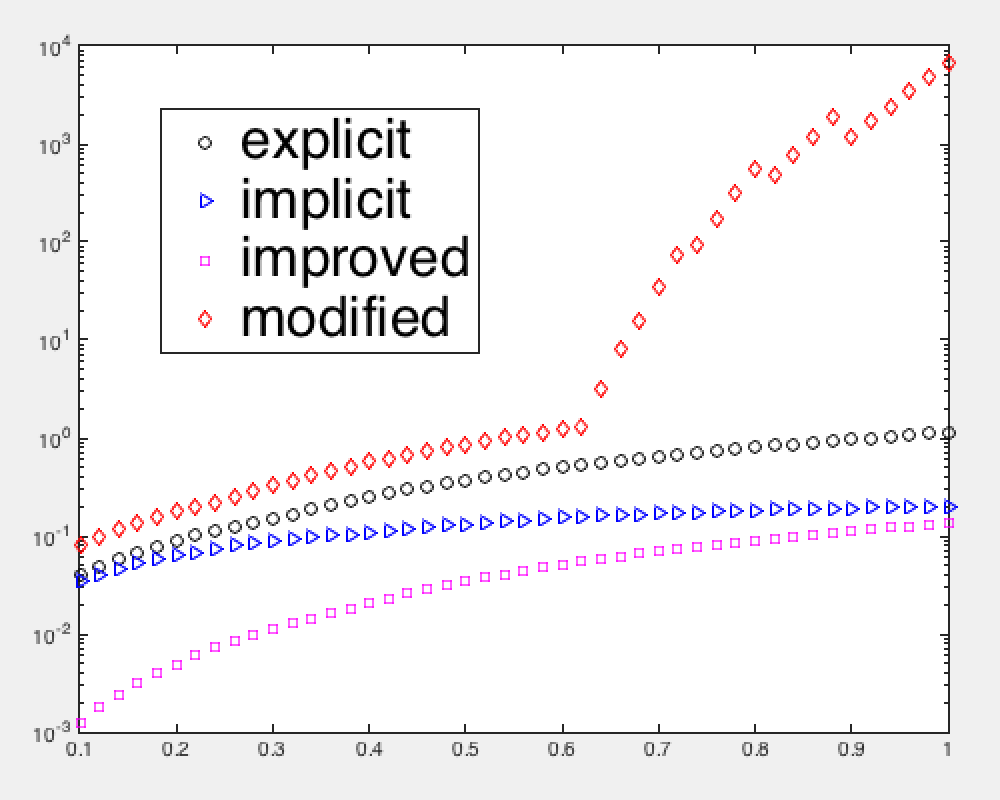
\includegraphics[width=\textwidth]{step-err-1.png}
        \caption{步长$\in [0.1, 1]$}
        \label{fig:boost}
    \end{subfigure}~
    \begin{subfigure}[t]{0.6\textwidth}
        \centering
        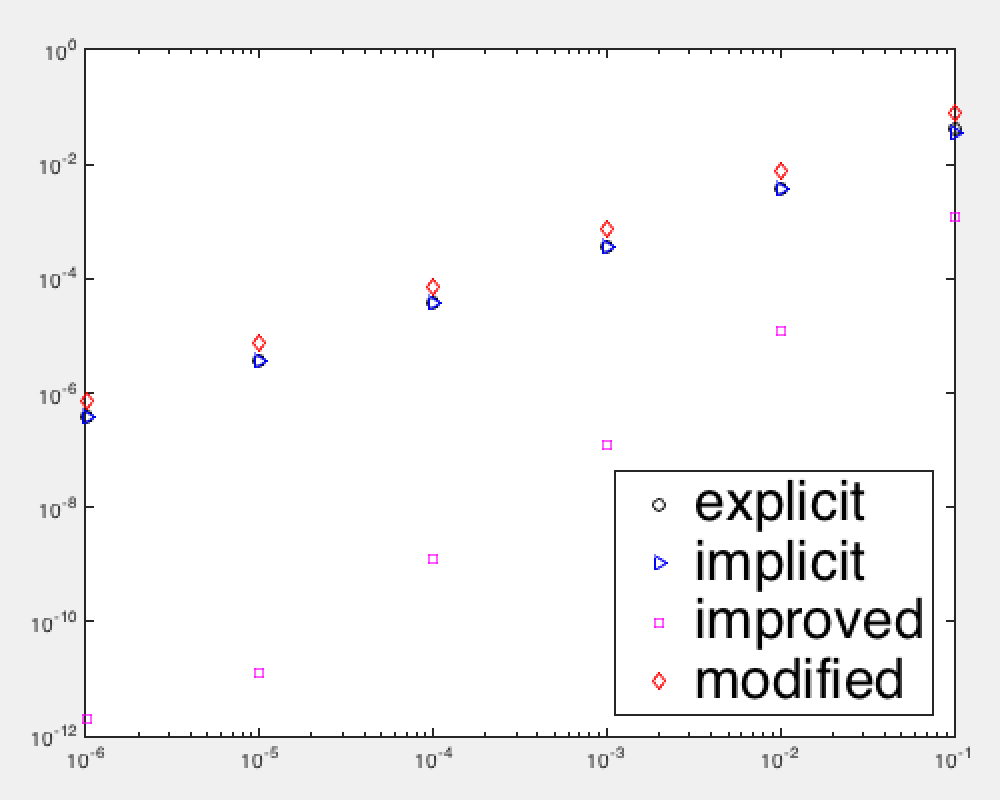
\includegraphics[width=\textwidth]{step-err-2.png}
        \caption{步长$\to 0$}
        \label{fig:accuracy}
    \end{subfigure}
    \caption{步长-误差关系图}
\end{figure}
可以看出四种格式误差均随步长减小而减小。其中修正的Euler格式在步长大于0.6多的时候会突然变得不稳定,误差以指数级爆炸增长(图\ref{fig:boost})。当步长不断趋近于0时,我们从图\ref{fig:accuracy}中可以看出,改进的Euler格式收敛阶数是其他三种格式的两倍,在步长为$10^{-6}$时误差已达到$10^{-12}$。

我选出几个具有代表性的步长:分别为0.9, 0.6, 0.3,可以看到修正的Euler格式由发散变为震荡收敛,再变为收敛。显式Euler格式在0.6的震荡和0.3的收敛也应证了后文对于显式格式绝对稳定区域的讨论。四种格式求得数值解与符号解对比如下:
\begin{figure}[H]
    \hspace{-6em}
    \begin{subfigure}[t]{0.42\textwidth}
        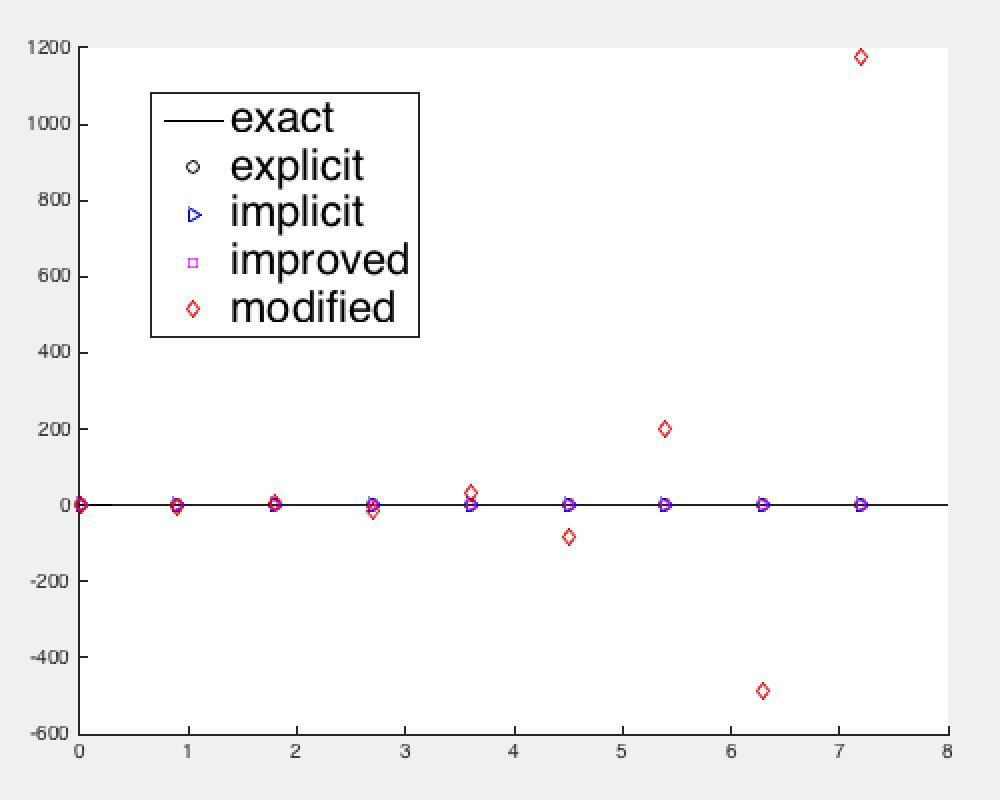
\includegraphics[width=\textwidth]{schemes-9.png}
        \caption{步长=0.9}
    \end{subfigure}~
    \begin{subfigure}[t]{0.42\textwidth}
        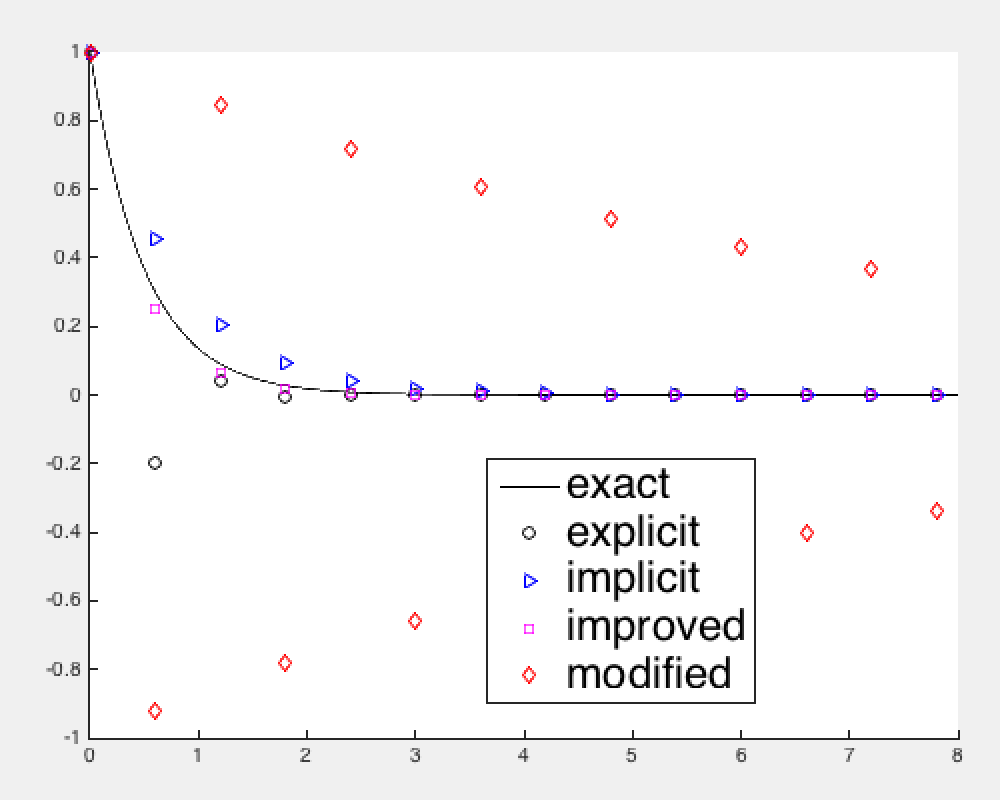
\includegraphics[width=\textwidth]{schemes-6.png}
        \caption{步长=0.6}
    \end{subfigure}~
    \begin{subfigure}[t]{0.42\textwidth}
        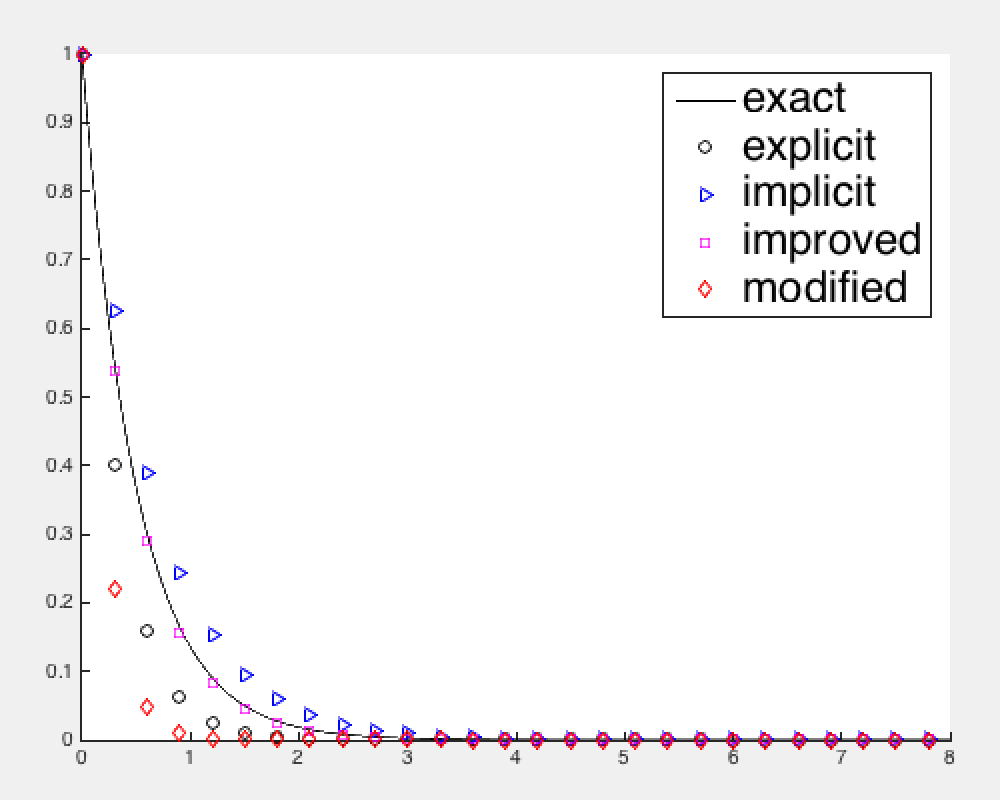
\includegraphics[width=\textwidth]{schemes-3.png}
        \caption{步长=0.3}
    \end{subfigure}
    \caption{不同步长下四种格式数值解与符号解对比}
\end{figure}
\section{给出修正和改进Euler格式的稳定性分析和绝对稳定区间(P73/1)}
\subsection{改进的Euler格式}
$$\text{由}~u_{n+1}=u_n+\frac{\Delta t}{2}\left(f_n+f_{n+1}\right)$$得到对于标准测试问题(Dahlquist测试问题)$\mathrm{d}u/\mathrm{d}t=au$,有$$u_{n+1}=\frac{1+\frac{a\Delta t}{2}}{1-\frac{a\Delta t}{2}}u_n,~u^\epsilon_{n+1}=\frac{1+\frac{a\Delta t}{2}}{1-\frac{a\Delta t}{2}}u^\epsilon_n.$$
$$\text{故}~\bigabs{u^\epsilon_{n+1}-u_{n+1}}=\left(\frac{1+\frac{a\Delta t}{2}}{1-\frac{a\Delta t}{2}}\right)\bigabs{u^\epsilon_n-u_n}=\cdots=\left(\frac{1+\frac{a\Delta t}{2}}{1-\frac{a\Delta t}{2}}\right)^n\bigabs{u^\epsilon_0-u_0}.$$
如果希望初始的舍入误差对固定的$\Delta t$,当$n\to\infty$时,仍然可以控制,则必须有:$$\bigabs{\frac{1+\frac{a\Delta t}{2}}{1-\frac{a\Delta t}{2}}}\leqslant1.$$
注意到因为$\Delta t>0$,所以上式成立当且仅当$a\leqslant0$,即此时改进的Euler格式对初始扰动稳定。

若令$z=a\Delta t$,则改进的Euler格式的绝对稳定区域为$$\bigabs{\frac{2+z}{2-z}}\leqslant1,~z\in\mathcal{Z},$$即实部为负的半复平面(图\ref{fig:imprv})
\subsection{修正的Euler格式}
$$\text{由}~u_{n+1}=u_n+\Delta tf\left(t_{n+\frac{1}{2}},u_n+\frac{\Delta t}{2}f_n\right)$$得到对于标准测试问题(Dahlquist测试问题)$\mathrm{d}u/\mathrm{d}t=au$,有$$u_{n+1}=\left(1+a\Delta t+\frac{(a\Delta t)^2}{2}\right)u_n,~u^\epsilon_{n+1}=\left(1+a\Delta t+\frac{(a\Delta t)^2}{2}\right)u^\epsilon_n.$$
$$\text{故}~\bigabs{u^\epsilon_{n+1}-u_{n+1}}=\left(1+a\Delta t+\frac{(a\Delta t)^2}{2}\right)\bigabs{u^\epsilon_n-u_n}=\cdots=\left(1+a\Delta t+\frac{(a\Delta t)^2}{2}\right)^n\bigabs{u^\epsilon_0-u_0}.$$
如果希望初始的舍入误差对固定的$\Delta t$,当$n\to\infty$时,仍然可以控制,则必须有:$$\bigabs{1+a\Delta t+\frac{(a\Delta t)^2}{2}}\leqslant1.$$
令$z=a\Delta t,$则修正的Euler格式绝对稳定区域如图\ref{fig:modfy}所示,即$$\bigabs{1+z+\frac{z^2}{2}}\leqslant1,~z\in\mathcal{Z}.$$
\begin{figure}[H]
    \hspace{-1em}
    \begin{subfigure}[t]{0.5\textwidth}
        \centering
        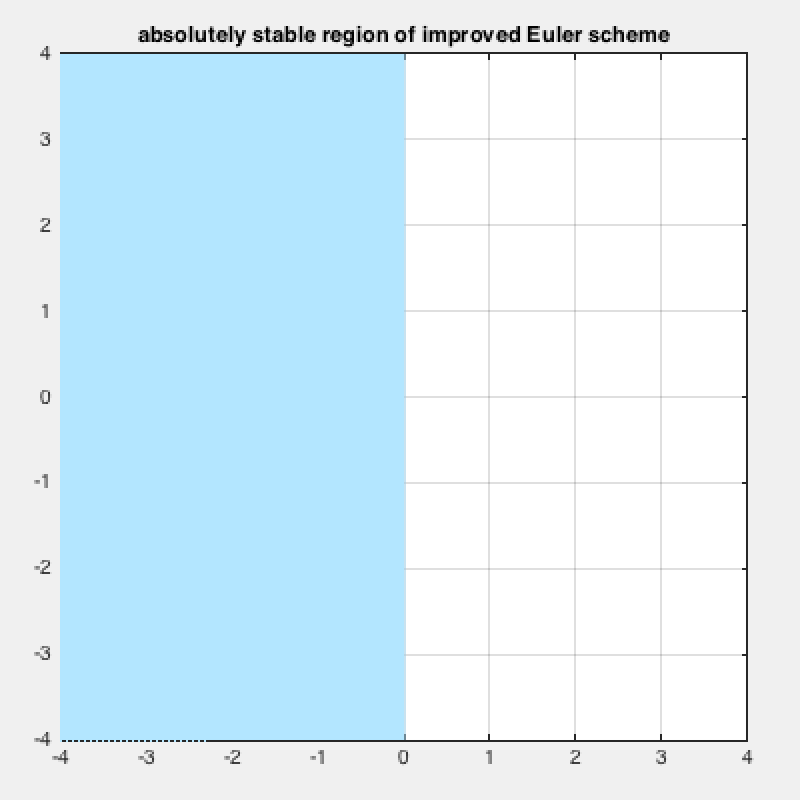
\includegraphics[width=\textwidth]{ASR-imprv.png}
        \caption{改进的Euler格式}
        \label{fig:imprv}
    \end{subfigure}~
    \begin{subfigure}[t]{0.5\textwidth}
        \centering
        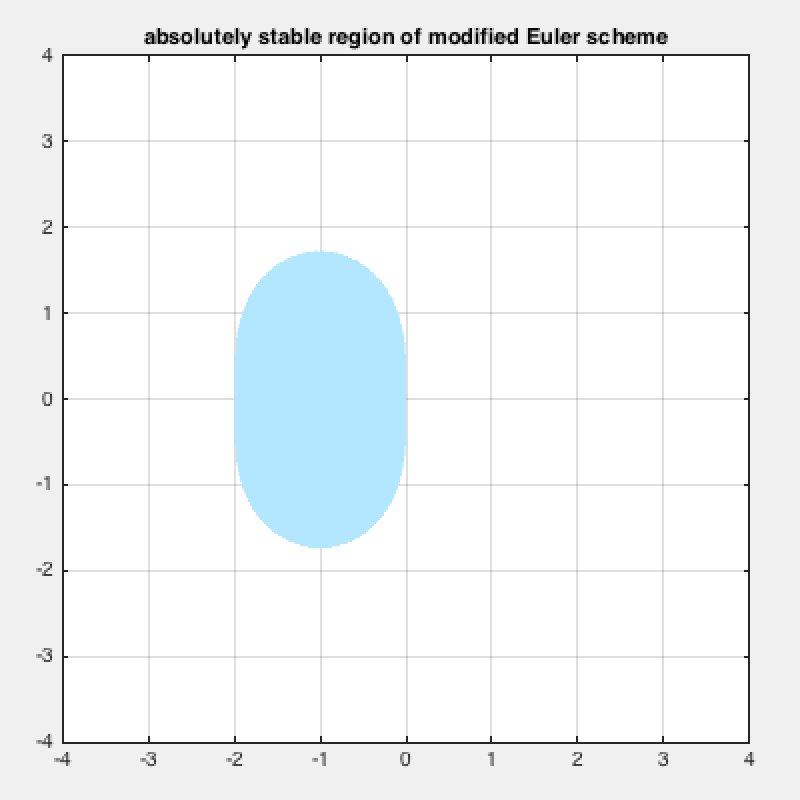
\includegraphics[width=\textwidth]{ASR-modfy.png}
        \caption{修正的Euler格式}
        \label{fig:modfy}
    \end{subfigure}
    \caption{绝对稳定区域}
    \label{ASR}
\end{figure}
\end{document}
